% !TeX program = pdflatex
% !TeX root = FourDivergence.tex

\documentclass[../FeynCalcManual.tex]{subfiles}
\begin{document}
\hypertarget{fourdivergence}{%
\section{FourDivergence}\label{fourdivergence}}

\texttt{FourDivergence[\allowbreak{}exp,\ \allowbreak{}FV[\allowbreak{}p,\ \allowbreak{}mu]]}
calculates the partial derivative of exp w.r.t \(p^{\mu }\).
\texttt{FourDivergence[\allowbreak{}exp,\ \allowbreak{}FV[\allowbreak{}p,\ \allowbreak{}mu],\ \allowbreak{}FV[\allowbreak{}p,\ \allowbreak{}nu],\ \allowbreak{}...]}
gives the multiple derivative.

\subsection{See also}

\hyperlink{toc}{Overview}, \hyperlink{threedivergence}{ThreeDivergence}.

\subsection{Examples}

\begin{Shaded}
\begin{Highlighting}[]
\NormalTok{SP}\OperatorTok{[}\FunctionTok{p}\OperatorTok{,} \FunctionTok{q}\OperatorTok{]} 
 
\NormalTok{FourDivergence}\OperatorTok{[}\SpecialCharTok{\%}\OperatorTok{,}\NormalTok{ FV}\OperatorTok{[}\FunctionTok{q}\OperatorTok{,} \SpecialCharTok{\textbackslash{}}\OperatorTok{[}\NormalTok{Mu}\OperatorTok{]]]}
\end{Highlighting}
\end{Shaded}

\begin{dmath*}\breakingcomma
\overline{p}\cdot \overline{q}
\end{dmath*}

\begin{dmath*}\breakingcomma
\overline{p}^{\mu }
\end{dmath*}

\begin{Shaded}
\begin{Highlighting}[]
\NormalTok{SP}\OperatorTok{[}\FunctionTok{p} \SpecialCharTok{{-}} \FunctionTok{k}\OperatorTok{,} \FunctionTok{q}\OperatorTok{]} 
 
\NormalTok{FourDivergence}\OperatorTok{[}\SpecialCharTok{\%}\OperatorTok{,}\NormalTok{ FV}\OperatorTok{[}\FunctionTok{k}\OperatorTok{,} \SpecialCharTok{\textbackslash{}}\OperatorTok{[}\NormalTok{Mu}\OperatorTok{]]]}
\end{Highlighting}
\end{Shaded}

\begin{dmath*}\breakingcomma
(\overline{p}-\overline{k})\cdot \overline{q}
\end{dmath*}

\begin{dmath*}\breakingcomma
-\overline{q}^{\mu }
\end{dmath*}

\begin{Shaded}
\begin{Highlighting}[]
\NormalTok{SFAD}\OperatorTok{[\{}\FunctionTok{p}\OperatorTok{,} \FunctionTok{m}\SpecialCharTok{\^{}}\DecValTok{2}\OperatorTok{\}]} 
 
\NormalTok{FourDivergence}\OperatorTok{[}\SpecialCharTok{\%}\OperatorTok{,}\NormalTok{ FVD}\OperatorTok{[}\FunctionTok{p}\OperatorTok{,} \SpecialCharTok{\textbackslash{}}\OperatorTok{[}\NormalTok{Nu}\OperatorTok{]]]}
\end{Highlighting}
\end{Shaded}

\begin{dmath*}\breakingcomma
\frac{1}{(p^2-m^2+i \eta )}
\end{dmath*}

\begin{dmath*}\breakingcomma
-\frac{2 p^{\nu }}{(p^2-m^2+i \eta )^2}
\end{dmath*}

\begin{Shaded}
\begin{Highlighting}[]
\NormalTok{FVD}\OperatorTok{[}\FunctionTok{l}\OperatorTok{,} \SpecialCharTok{\textbackslash{}}\OperatorTok{[}\NormalTok{Mu}\OperatorTok{]]}\NormalTok{ FAD}\OperatorTok{[\{}\FunctionTok{l}\OperatorTok{,} \DecValTok{0}\OperatorTok{\},} \OperatorTok{\{}\FunctionTok{l} \SpecialCharTok{{-}} \FunctionTok{p}\OperatorTok{,} \DecValTok{0}\OperatorTok{\}]} 
 
\NormalTok{FourDivergence}\OperatorTok{[}\SpecialCharTok{\%}\OperatorTok{,}\NormalTok{ FVD}\OperatorTok{[}\FunctionTok{l}\OperatorTok{,} \SpecialCharTok{\textbackslash{}}\OperatorTok{[}\NormalTok{Mu}\OperatorTok{]]]}
\end{Highlighting}
\end{Shaded}

\begin{dmath*}\breakingcomma
\frac{l^{\mu }}{l^2.(l-p)^2}
\end{dmath*}

\begin{dmath*}\breakingcomma
\frac{D}{l^2.(l-p)^2}-\frac{2 l^2}{\left(l^2\right)^2.(l-p)^2}+\frac{2 (l\cdot p)-2 l^2}{l^2.(l-p)^4}
\end{dmath*}

\begin{Shaded}
\begin{Highlighting}[]
\NormalTok{SP}\OperatorTok{[}\FunctionTok{p}\OperatorTok{,} \FunctionTok{w}\OperatorTok{]}\SpecialCharTok{*}\NormalTok{SpinorUBar}\OperatorTok{[}\NormalTok{p2}\OperatorTok{,} \FunctionTok{m}\OperatorTok{]}\NormalTok{ . GS}\OperatorTok{[}\FunctionTok{w}\OperatorTok{]}\NormalTok{ . SpinorU}\OperatorTok{[}\NormalTok{p1}\OperatorTok{,} \FunctionTok{m}\OperatorTok{]} 
 
\NormalTok{FourDivergence}\OperatorTok{[}\SpecialCharTok{\%}\OperatorTok{,}\NormalTok{ FV}\OperatorTok{[}\FunctionTok{w}\OperatorTok{,} \FunctionTok{a}\OperatorTok{]]}
\end{Highlighting}
\end{Shaded}

\begin{dmath*}\breakingcomma
\left(\overline{p}\cdot \overline{w}\right) \bar{u}(\text{p2},m).\left(\bar{\gamma }\cdot \overline{w}\right).u(\text{p1},m)
\end{dmath*}

\begin{dmath*}\breakingcomma
\left(\overline{p}\cdot \overline{w}\right) \left(\varphi (\overline{\text{p2}},m)\right).\bar{\gamma }^a.\left(\varphi (\overline{\text{p1}},m)\right)+\overline{p}^a \left(\varphi (\overline{\text{p2}},m)\right).\left(\bar{\gamma }\cdot \overline{w}\right).\left(\varphi (\overline{\text{p1}},m)\right)
\end{dmath*}

Differentiation of \(4\)-vectors living in different dimensions (\(4\),
\(D\), \(D-4\)) works only in the t'Hooft-Veltman scheme

\begin{Shaded}
\begin{Highlighting}[]
\NormalTok{FourDivergence}\OperatorTok{[}\NormalTok{FVD}\OperatorTok{[}\FunctionTok{p}\OperatorTok{,}\NormalTok{ mu}\OperatorTok{],}\NormalTok{ FV}\OperatorTok{[}\FunctionTok{p}\OperatorTok{,}\NormalTok{ nu}\OperatorTok{]]}
\end{Highlighting}
\end{Shaded}

\begin{figure}[!ht]
\centering
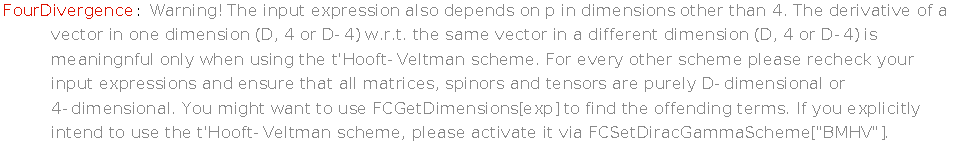
\includegraphics[width=0.6\linewidth]{img/0n13hj2mmcy3r.pdf}
\end{figure}

\begin{dmath*}\breakingcomma
\text{\$Aborted}
\end{dmath*}

\begin{Shaded}
\begin{Highlighting}[]
\NormalTok{FCSetDiracGammaScheme}\OperatorTok{[}\StringTok{"BMHV"}\OperatorTok{]}\NormalTok{;}
\end{Highlighting}
\end{Shaded}

\begin{Shaded}
\begin{Highlighting}[]
\NormalTok{FourDivergence}\OperatorTok{[}\NormalTok{FVD}\OperatorTok{[}\FunctionTok{p}\OperatorTok{,}\NormalTok{ mu}\OperatorTok{],}\NormalTok{ FV}\OperatorTok{[}\FunctionTok{p}\OperatorTok{,}\NormalTok{ nu}\OperatorTok{]]}
\end{Highlighting}
\end{Shaded}

\begin{dmath*}\breakingcomma
\bar{g}^{\text{mu}\;\text{nu}}
\end{dmath*}
\end{document}
